\RequirePackage{etex}
\RequirePackage{fix-cm} % For custom font shaping

% Document class
\documentclass[pdftex, 11pt, a4paper, oneside, english]{memoir}

% Page styling
\let\footruleskip\undefined
\usepackage{fancyhdr}
\pagestyle{fancy}

% English language package
\usepackage[english]{babel}

% UTF-8 characters
\usepackage[utf8]{inputenc}

% Package for dummy text
\usepackage{lipsum}

%Packages for writing algorithms nicely
\usepackage{algorithm}
\usepackage{algpseudocode}

% Colors for chapters and table of content
\usepackage[table,xcdraw]{xcolor}
\definecolor{ThemeColor}{RGB}{51, 102, 255} % Blue
\definecolor{BlackColor}{RGB}{0, 0, 0} % Black

% Table packages
% Merge cells i tables
\usepackage{multirow}
\usepackage{makecell}
\usepackage{tabularx}

% PDF propeties (fx. hyperlinks, pdftitle)
\usepackage[hyphens]{url}
\usepackage[bookmarks=true,bookmarksnumbered=true,citecolor=black,colorlinks=true,hyperfigures=true,hyperfootnotes=true,hyperindex=true,linkcolor=black,urlcolor=blue]{hyperref}

% BibTeX = bibliography
% ALWAYS USE \citep{} or something like:
% \citep[see this baws article]{fooArticle}
%\usepackage[semicolon,authoryear,round]{natbib}
%\bibliographystyle{plainnat}
%vancover standard 
\usepackage[square,numbers]{natbib}
\bibliographystyle{abbrvnat}

%for including pdfs in the report
\usepackage{pdfpages}
% Package for editing captions. Fx for figures and code listings
\usepackage[textfont={footnotesize,sl}]{caption}

%Package for MATLAB code
\usepackage[framed, numbered]{mcode}

% Package for more elegant math
\usepackage{amsmath}
\usepackage{xfrac} % for \sfrac command


% Styles
% Package for setup of chapters and sections
\usepackage{titlesec}


% % % % % % % % % % % % % % CHAPTER  % % % % % % % % % % % % % % % % % % % % % %
% Define fontsize for the numbering of the chapters
\newcommand{\ChapterNumbering}{
    \usefont{\encodingdefault}{\rmdefault}{b}{n}
    \fontsize{35}{45}\normalfont\color{ThemeColor}}

% Chapter numbers in margin
\chapterstyle{hangnum}

% Modifying "\chapterstyle{hangnum}"
% Changing vertical position of chapter headline
\renewcommand*{\chapterheadstart}{\vspace*{-20pt}}

% Color setup for chapters
% Title color
\renewcommand*{\chaptitlefont}{\bfseries\Huge\color{BlackColor}}
% Number color
\renewcommand{\chapnumfont}{\normalfont\ChapterNumbering\color{ThemeColor}}




% % % % % % % % % % % % % % SECTION  % % % % % % % % % % % % % % % % % % % % % %
% Section numbers in margin
\hangsecnum

% Color setup for sections
% Title color
%\renewcommand\thesection{\color{ThemeColor}\thechapter.\arabic{section}}
\renewcommand\thesection{\thechapter.\arabic{section}}

% Set numbering depth of sections
\setsecnumdepth{subsubsection}

% Set the depth of sections included in table of contents
\settocdepth{subsection}



% Clear all header an footer fields
\fancyhf{}


% % % % % % % % % % % % % % HEADER % % % % % % % % % % % % % % % % % % % % % % %
% Delete headruler
\renewcommand{\headrulewidth}{0pt}

% Insert picture in left side on even pages and right side on odd pages
%\fancyhead[R]{
\includegraphics[height=40pt]{figure/header/header}}



% % % % % % % % % % % % % % FOOTER % % % % % % % % % % % % % % % % % % % % % % %
% Insert pagenumber on right side of even page, left side of odd page
\fancyfoot[R]{\thepage}

\setlength\headheight{44.1pt}

%\setcounter{page}{1}

%%%%%%%%%%%%%%%%%%%%%%%%%%%%%%%%%%%%%%%%%%%%%%%%%%%%%%%%%%%%%%%%%%%%%%%%%%%%%%%%
%                       Custom for figures (myFigure etc.)                     %
%                     			      	        		                       %
%%%%%%%%%%%%%%%%%%%%%%%%%%%%%%%%%%%%%%%%%%%%%%%%%%%%%%%%%%%%%%%%%%%%%%%%%%%%%%%%

% Include image and graphic
\usepackage{graphicx}

% Package for wrapping figures in text
\usepackage{wrapfig}

% Set the path where LaTeX looks for pictures.
\graphicspath{{figure/}}

% You need a newsubfloat element to use subcaption
\newsubfloat{figure}

% Command to set caption styles
\captionsetup[figure]{
    labelfont=bf
}

\captionsetup[table]{
    labelfont=bf
}

% from the old preamble
\captionnamefont{\bfseries\small}
\captiontitlefont{\itshape\small}
\subcaptionlabelfont{\bfseries\small}
\subcaptionfont{\itshape\small}


% Command \myFigure{filename}{caption}{label}{width} 
% for inserting a new figure.
\newcommand{\myFigure}[4]
{ 
    \begin{figure}[ht] 
        \centering 
        \includegraphics[width=#4\textwidth]{#1} 
        \caption{#2} 
        \label{#3} 
    \end{figure}
} 

\newcommand{\myFigureWithRotation}[5]
{ 
	\begin{figure}[ht] 
		\centering 
		\includegraphics[width=#4\textwidth, angle=#5]{#1} 
		\caption{#2} 
		\label{#3} 
	\end{figure}
} 
 
% Insert a figure wraped in text (left/right)
% Command \myWrapFigure{filename}{caption}{label}{width}{r/l}
\newcommand{\myWrapFigure}[5]
{ 
    \begin{wrapfigure}{#5}{#4 \textwidth}
        \begin{center}
            \includegraphics[width=#4\textwidth]{#1}
        \end{center}
        \caption{#2}
        \label{#3} 
    \end{wrapfigure}
}
 
% Insert two figures side by side, with a caption covering both and a subcaption for each figure. OBS: scaled for 50 % text width both
% Command \mySubFigure{filename1}{filename2}{caption}
% {subcaption1}{subcaption2}{label}{sublabel1}{sublabel2}
\newcommand{\mySubFigure}[9]
{
    \begin{figure}[ht]
        \centering
        \subbottom[{#4}\label{#7}]%
            {\includegraphics[width=0.47\textwidth]{#1}}\hfill
        \subbottom[{#5}\label{#8}]%
            {\includegraphics[width=0.47\textwidth]{#2}}
        \caption{#3}
        \label{#6}
    \end{figure}
}

%\mySubFigure{filename1}{filename2}{filename3}{caption}
% {subcaption1}{subcaption2}{subcaption2}{label}{sublabel1}{sublabel2}{sublabel3}
\newcommand{\mySubFigures}[9]
{
	\begin{figure}[ht]
		\centering
		\subbottom[{#4}\label{#7}]%
			{\includegraphics[width=0.33\textwidth]{#1}}\hfill
		\subbottom[{#5}\label{#8}]%
			{\includegraphics[width=0.33\textwidth]{#2}}
		\subbottom[{#6}\label{#9}]%
			{\includegraphics[width=0.33\textwidth]{#1}}\hfill
		\caption{#3}
		\label{#6}
	\end{figure}
}


% Keeps floats in the section. 
% Help control place to put pix
\usepackage[section]{placeins}


%Package with enumirate command with extra options (used within cells of tabular)
\usepackage[inline]{enumitem}
\usepackage[]{todonotes}


% new commands for individually colored todo 
\newcommand{\todosimon}[2]{
\todo[#1, color=blue!40]{#2 \\- Simon}
}

\newcommand{\todorene}[2]{
\todo[#1, color=green!40]{#2 \\- Rene}
}

\newcommand{\todoivan}[2]{
	\todo[#1, color=green!40]{#2 \\- Ivan}
}

\newcommand{\todotorben}[2]{
	\todo[#1, color=green!40]{#2 \\- Torben}
}
\usepackage[utf8]{inputenc}

% Default fixed font does not support bold face
\DeclareFixedFont{\ttb}{T1}{txtt}{bx}{n}{8} % for bold
\DeclareFixedFont{\ttm}{T1}{txtt}{m}{n}{8}  % for normal


\definecolor{deepblue}{rgb}{0,0,0.5}
\definecolor{deepred}{rgb}{0.6,0,0}
\definecolor{deepgreen}{rgb}{0,0.5,0}

\usepackage{listings}

% Python style for highlighting
\newcommand\pythonstyle{\lstset{

}}


%New colors defined below
\definecolor{codegreen}{rgb}{0,0.6,0}
\definecolor{codegray}{rgb}{0.5,0.5,0.5}
\definecolor{codepurple}{rgb}{0.58,0,0.82}
\definecolor{backcolour}{rgb}{0.95,0.95,0.92}

%Code listing style named "mystyle"
\lstdefinestyle{python}{
	%keepspaces=true,
	language=python,
	showtabs=true,
	tab=,
	tabsize=2,
	basicstyle=\ttfamily\footnotesize,%\setstretch{.5},
	stringstyle=\color{stringcolour},
	showstringspaces=false,
	alsoletter={1234567890},
	otherkeywords={\%, \}, \{, \&, \|},
	keywordstyle=\color{keywordcolour}\bfseries,
	emph={and,break,class,continue,def,yield,del,elif ,else,%
		except,exec,finally,for,from,global,if,import,in,%
		lambda,not,or,pass,print,raise,return,try,while,assert,with},
	emphstyle=\color{blue}\bfseries,
	emph={[2]True, False, None},
	emphstyle=[2]\color{keywordcolour},
	emph={[3]object,type,isinstance,copy,deepcopy,zip,enumerate,reversed,list,set,len,dict,tuple,xrange,append,execfile,real,imag,reduce,str,repr},
	emphstyle=[3]\color{commandcolour},
	emph={Exception,NameError,IndexError,SyntaxError,TypeError,ValueError,OverflowError,ZeroDivisionError},
	emphstyle=\color{exceptioncolour}\bfseries,
	%upquote=true,
	morecomment=[s]{"""}{"""},
	commentstyle=\color{commentcolour}\slshape,
	%emph={[4]1, 2, 3, 4, 5, 6, 7, 8, 9, 0},
	emph={[4]ode, fsolve, sqrt, exp, sin, cos,arctan, arctan2, arccos, pi,  array, norm, solve, dot, arange, isscalar, max, sum, flatten, shape, reshape, find, any, all, abs, plot, linspace, legend, quad, polyval,polyfit, hstack, concatenate,vstack,column_stack,empty,zeros,ones,rand,vander,grid,pcolor,eig,eigs,eigvals,svd,qr,tan,det,logspace,roll,min,mean,cumsum,cumprod,diff,vectorize,lstsq,cla,eye,xlabel,ylabel,squeeze},
	emphstyle=[4]\color{numpycolour},
	emph={[5]__init__,__add__,__mul__,__div__,__sub__,__call__,__getitem__,__setitem__,__eq__,__ne__,__nonzero__,__rmul__,__radd__,__repr__,__str__,__get__,__truediv__,__pow__,__name__,__future__,__all__},
	emphstyle=[5]\color{specmethodcolour},
	emph={[6]assert,yield},
	emphstyle=[6]\color{keywordcolour}\bfseries,
	emph={[7]range},
	emphstyle={[7]\color{keywordcolour}\bfseries},
	% emph={[7]self},
	% emphstyle=[7]\bfseries,
	literate=*%
	{:}{{\literatecolour:}}{1}%
	{=}{{\literatecolour=}}{1}%
	{-}{{\literatecolour-}}{1}%
	{+}{{\literatecolour+}}{1}%
	{*}{{\literatecolour*}}{1}%
	{**}{{\literatecolour{**}}}2%
	{/}{{\literatecolour/}}{1}%
	{//}{{\literatecolour{//}}}2%
	{!}{{\literatecolour!}}{1}%
	%{(}{{\literatecolour(}}{1}%
	%{)}{{\literatecolour)}}{1}%
	{[}{{\literatecolour[}}{1}%
	{]}{{\literatecolour]}}{1}%
	{<}{{\literatecolour<}}{1}%
	{>}{{\literatecolour>}}{1}%
	{>>>}{\pythonprompt}{3}%
	,%
	%aboveskip=.5ex,
	frame=trbl,
	%frameround=tttt,
	%framesep=.3ex,
	rulecolor=\color{black!40},
	%framexleftmargin=\framemargin,
	%framextopmargin=.1ex,
	%framexbottommargin=.1ex,
	%framexrightmargin=\framemargin,
	%framexleftmargin=1mm, framextopmargin=1mm, frame=shadowbox, rulesepcolor=\color{blue},#1
	%frame=tb,
	backgroundcolor=\color{white},
	breakindent=.5\textwidth,frame=single,breaklines=true%
	%}
}
%%%%%%%%%%%%%%%%%%%%%%%%%%%%%%%%%%%%%%%%%%%%%%%%%%%%%%%%%%%%%%%%%%%%%%%%%%%%%%%%
%                           Custom Commands                                    %
%                                                                              %
%%%%%%%%%%%%%%%%%%%%%%%%%%%%%%%%%%%%%%%%%%%%%%%%%%%%%%%%%%%%%%%%%%%%%%%%%%%%%%%%

%%%%% FIGURES %%%%%
% The following commands are defined in: style/figure

% Insert a new figure:
% \myFigure{filename}{caption}{label}{width}
% width is ratio of textwidth, so it should be between 0.1 and 1

% Insert a figure wraped in text (left/right)
% \myWrapFigure{filename}{caption}{label}{width}{l/r}
% width is ratio of textwidth, so it should be between 0.1 and 1
% l/r: l = left, r = right

% Insert two figures side by side, with a caption covering both and a subcaption for each figure. OBS: scaled for 50 % text width both
% Command \mySubFigure{filename1}{filename2}{caption}
% {subcaption1}{subcaption2}{label}{sublabel1}{sublabel2}



%%%%% TABLES %%%%%
% Command \myTable{caption text}{refrence label}{input filename: eq <tables/myTable>}
% for inserting tables


%%%%% CODE LISTING %%%%%
%\begin{lstlisting}[language=Matlab, caption={Dette er et eksempel på hvordan du skal bruge listing}, label=list_me_like_a_baws]
%
%	INSERT CODE HERE
%
%\end{lstlisting}

% For more info go to http://ctan.org/pkg/listing



%%%%% EQUATIONS / MATH %%%%%
% For info in the user guide at http://ctan.org/pkg/amsmath
% Feel free to add ninja tricks to this guide



%%%%% BibTeX %%%%%
% To cite some article use:
% \citep{fooArticle} or
% \citep[see this baws article]{fooArticle}

% OBS: remember to add article to "bibliografi.bib" using syntex of the examples in the file.



%%%%% Nomenclature %%%%%
% When introducing a new symbol add it to the nomenclature by:
% \nomenclature{symbol}{description}
% remember to put symbol in mathmode if necessary
% OBS: if you need to add more the one symbol you have to add a "%" at the end of every \nomenclature use except for the last one. See example below:
%
%	\begin{equation}
%		e=m \cdot c^2
%	\end{equation}%
%	\nomenclature{$e$}{Energy}%
%	\nomenclature{$m$}{The mass}%
%	\nomenclature{$c$}{The speed of light. 299 792 458 $\frac{m}{s}$}

%%%%% COLOR %%%%%
\definecolor{deadlinecolor}{HTML}{FD6864}
\definecolor{reviewcolor}{HTML}{9698ED}

%%%%% TEXT COMMANDS %%%%%
\newcommand{\prbl}{Problematic} % For the lulz

%%%%% MATH COMMANDS %%%%%
\newcommand{\degree}{^\circ}

% Command \myTable{caption text}{refrence label}{input filename: eq <tables/myTable>}
% for inserting tables
\newcommand{\myTable}[3]
{ 
    \begin{table}[h]
    \centering
    \caption{#1}
    \label{#2}
        \input{#3}
    \end{table}
}
% Example on content in table file
%
%    \begin{tabular}{rll}
%    \multicolumn{1}{c}{\textbf{Tapsstørrelse}} &
%    \multicolumn{1}{c}{\textbf{Målt beregningstid}} \\ \hline
%       1      &  35,6  $\mu s$     \\[0.05cm] 
%       2      &  36,5  $\mu s$     \\[0.05cm] 
%       5      &  32,0  $\mu s$     \\[0.05cm] 
%       8      &  32,0  $\mu s$     \\[0.05cm] 
%       10     &  32,0  $\mu s$     \\[0.05cm] 
%       20     &  32,5  $\mu s$     \\[0.05cm] 
%       50     &  69,0  $\mu s$     \\[0.05cm] 
%       80     &  101,5 $\mu s$     \\[0.05cm] 
%       100    &  124,5 $\mu s$     \\[0.05cm] 
%       200    &  240,5 $\mu s$     \\[0.05cm] 
%       500    &  587   $\mu s$     \\[0.05cm] 
%       800    &  932   $\mu s$     \\[0.05cm] 
%       1000   &  1164  $\mu s$     \\[0.05cm] 
%       1024   &  1192  $\mu s$     \\[0.05cm]
%       \hline
%       512    &  601   $\mu s$     \\[0.05cm]
%       513    &  605   $\mu s$     \\
%    \end{tabular}



% Geometry for frontpage
\usepackage{geometry}

% For traceability matrix
\usepackage{longtable}
\usepackage{rotating}

\usepackage{subcaption}
\usepackage{tabularx}


\AtBeginDocument{\renewcommand\contentsname{Contents \vspace{-1.5em}}}

\addtocontents{toc}{\protect\setcounter{tocdepth}{1}}



\begin{document}

	\begin{titlingpage}
		% Frontpage goes here
		\newgeometry{left=3cm,bottom=0.1cm}

\centerline{\Huge\bfseries\color{ThemeColor} Deep learning project}

\vspace{5em}
\centerline{\large\bfseries\color{BlackColor}}
\vspace{0.5em}
\centerline{\large\color{BlackColor}Department of Engineering - Aarhus University}

\vspace{0.5em}
\centerline{\large\color{BlackColor} June 3, 2017}



\vspace{25em}

\begin{center}
   \begin{tabular}{ l p{3cm} l l }
    Stud. no.: 201270782 && Torben Werenberg Vogt & \\\hline
	& & \\
	Stud. no.: 201270097 && Simon Østergaard Kristensen & \\\hline
	& & \\
	Stud. no.: 201270278 && Ivan Bjerring Hansen & \\\hline
   \end{tabular}
\end{center}
\thispagestyle{empty} % No header and footer on this page
\restoregeometry


	\end{titlingpage}

    % Table of contents
	\tableofcontents*
	
	\chapter{Introduction}
\label{chp:intro}

This report is a description of the project conducted as part of the mandatory work in the course Deep Learning at Aarhus University Department of Engineering.

In the project, a neural network will be constructed with the purpose of training and testing on the Cifar-10 data set. One network architecture is used, but different hyperparameters will be presented as to show how tweaking these can drastically alter the results of the neural networks performance. 

The theory behind the project will be presented as well. This theory is part of the curriculum of the course, and gives the necessary knowledge to understand the developed neural network. 

The project is developed in Python 3.5 in a Tensorflow environment. Tensorboard is used for visualizing results. 
	\chapter{Applied theory}
\label{chp:theory}

\section{Convolutional network layers}
Traditional neural network with fully-connected layers does not perform well with images classification. This is because they create the number of weights due to the size of the image. For instance if an input image is 800x600x3 (wide, height, depth) the number of weights would be $800 * 600 * 3 = 1,440,000$. Due to the large number of parameters, it is easy to se that this is wasteful technique to work with images and furthermore it will lead to an overfitting of the input images. On the other hand a
Convolutional nerual network also called \emph{CNN} would be a better solution when working on images classification because it assumes that the input is an image or on the same form. The power in CNN is that the layers are three dimensional and the neurons can share weights and bias values. This reduces the amount of parameters significantly. The CNN consist of three different layers, namely a \emph{convolutional layer}, a \emph{pooling layer} and a \emph{fully-connected layer}. These three layers will be described in the following sections.

\subsection{Convolutional layer}
This is the layer where most is happening. The convolutional layer creates a number of filters with a height, width and a depth. Normally values for the height and width is three or five. The depth should be the same as the input image. So a dimension for filter for a 32x32x3 input image could be 5x5x3. Each filter looks at different things in the image eg. oriented edges, blotchs or colors. Each filter is convolve across the input image along the height and width. To specify how it has to convolve three hyperparameters need to be set namely \emph{depth}, \emph{stride} and \emph{zero-padding}. Depth is the number of neurons that looks at the same filter. Stride is the number of pixels the filter should convolve with across the image. Finally zero-padding is used to determine the size of the output volume. This is often the same as the input image. 

\subsection{Pooling layer}
Pooling layers are a type of layer that can be implemented in-between convolutional layers described in the section above. Their function is to down-sample the input by using a \emph{stride} and a \emph{window size} and is most often done by \emph{max pooling}. 

Max pooling works by using a filter of a specific size to choose the maximum value, and thereby down-sample. The size of the filter is determined by the window size. The stride is the step size that the filter slides over the input values with. This is illustrated in figure \ref{fig:pooling}, where the stride is set to 2 and the window size is set to 2x2. The filter then moves over the input by first choosing a maximum value inside its area, so for the red area the maximum value is 6, which is then put into the new matrix. The filter will then move two steps because of the stride and then choose a new maximum value. 

\myFigure{pooling.PNG}{Pooling layer \citep{NN3}}{fig:pooling}{0.5}

Since the pooling layer deals in down-sampling the original input, it helps control overfitting of the data. 

\subsection{Fully-connected layer}
A layer where all neurons are connected with all neuron in the previous layer is a \emph{fully-connected layer} compared to the convolutional layer  where they only are connected with the neurons in the filters and the neurons in a fully-connected layer can not share parameters.
This graphical illustration of a fully-connected layer can be seen in figure \ref{fig:fully_con}

\myFigure{fully-connected_layer.PNG}{Fully-connected layer \citep{FCL}}{fig:fully_con}{0.5}


\section{Optimization}
Optimization is closely related to the loss function, which evaluates the quality of any particular set of weights W. When doing optimization one actually tries to find weights so that the loss function is minimized. There are many different types of optimizers, however in this course the focus will be on the chosen Adam optimizer. 

\subsection{Adam optimizer}
Adaptive Moment Estimation or \emph{Adam} is a lot like RMSProp, which is a very effective adaptive learning rate method, however with the addition of momentum. In practice Adam often works slightly better than RMSProp, and according to cs231n it is currently recommended as the default \citep{NN3}. Adam also adds bias-correction, so that when a bias is added to the weights, the optimizer takes this into account. 


\section{Hyperparameters}
Hyperparameters are variables set before running one's neural network. They are inputs that can be tweaked in order to optimize the model. There are a lot of different hyperparameters to tweak when building a neural network, and in the following sections the hyperparameters that were focused on in this project are described. 


\subsection{Learning rate}
The learning rate is how quickly a network replaces old beliefs with new ones. An example could be a child learning about cars. If the first 10 cars the child sees are red, then it will believe cars are red and therefore look for red when needing to identify a car. If the child then begins seeing blue cars, then the learning rate determines how fast the child realizes that the red colour is not the most important characteristic of a car. A high learning rate results in fast realization, meaning the network will quickly change its mind. So while one would want a network that quickly can learn new characteristics, it is noteworthy that the learning rate can also be too high, which would result in fluctuating beliefs, and not make the model very precise. 

\myFigure{learning_rates.PNG}{Different learning rates \citep{NN3}}{fig:learning_rates}{0.5}

The effect of different learning rates can be seen in figure \ref{fig:learning_rates}. It is clear that the curve named \emph{good learning rate} is preferable, since it steadily approaches its minimum and flattens. The \emph{low learning rate} curve has the same tendency, however it is a lot slower and it will therefore take more time to get as good results. The \emph{high learning rate} curve reaches its minimum quickly and then flattens. However, despite initially getting a lower loss than the \emph{good learning rate} it does not reach as good a minimum in the end. The \emph{very high learning rate} curve ends up with a worse loss than it started with. This is because the parameters are bouncing around chaotically, meaning they are unable to settle in a nice spot. 

\subsection{Regulariation}
Regularization techniques generally prevents overfitting the model to the training data. The training and validation accuracy can be used to evaluate if the model is overfitting. This can be seen on figure \ref{fig:train_valid_acc}. In general there should be little difference between training and validation accuracy.

\myFigure{traina_valid_acc.PNG}{training and validation accurcay in relation to overfitting \citep{NN3}}{fig:train_valid_acc}{0.5}


\subsubsection{L2 regularization}
L2 regularization is one of the most common regularization techniques. The equation for calculating L2 regularization loss for every weight in the network can be written as illustrated in (2.1). 

\begin{equation}
\dfrac{1}{2} * \lambda * \omega^2
\end{equation}

It can be read from the equation that $\omega^2$ ensures that high peaky weights are penalized heavier than diffuse weights. L2 regularization therefore encourages utilizing all inputs even though it might give the same data loss as only utilizing few inputs. Experience shows that diffuse weights yield a better result \citep{LC_cs231n}.

When using L2 regularization the calculated regularization loss is added to the data loss. It is important not to overwhelm the data loss, so that the gradient primarily comes from the regularization loss instead of the data loss. 


\subsubsection{Dropout}
Dropout is an effective and simple regularization technique, complimenting other methods, such as the L2 regularization described in the section above. 

Dropout works by only keeping neurons active with a certain probability while training. So as shown in figure \ref{fig:dropout} the neurons are not necessarily all active. On the left side all neurons are active and connected, but on the right side seven of the neurons are deactivated causing less overfitting.  

\myFigure{dropout.PNG}{Dropout principle \citep{NN2}}{fig:dropout}{0.6}

The reason it causes less overfitting is that when the neurons used for training are varying, then the training will vary as well, meaning the model will not adapt too much to a specific belief. 

\subsubsection{Filter size}
When modifying one's convolutional layers, one of the tweakable hyperparameters is the filter size. Popular values are 3x3 or 5x5 \citep{FCL}. The filter size has to do with how the features of images are believed to be seen. A low filter size of for example 1x1 means that the filter only looks at one value for every stride. A low filter size is good for detecting smaller features in images. However, if the small features are not interesting for the classification, then it can be better to use a larger filter size, so that it will not focus on the wrong features. 








	\chapter{Implementation}
\label{chp:imp}
	\chapter{Results}
\label{chp:res}

This chapter describes the results of the implemented convolutional neural network applied to the CIFAR-10 dataset. It further presents the results of adjusting the hyperparameters: learning rate, L2 regularization, dropout and filter size.

First a coarse grain search was done followed by a fine grain search. These are both done with the network architecture illustrated in figure \ref{fig:conv_arch}. Finally the network architecture illustrated in figure \ref{fig:deep} is evaluated with one set of hyperparameters. 

\section{Coarse grain  search}
The coarse grain search is applied to identity a reasonable range for the different hyperparameters.

\subsection{Learning rate}
Based on the default learning rate of Adam being 0.001 it was chosen to do 3 runs and investigate the loss function. The three learning rates were: 0.01, 0.001 and 0.0001. The three graphs are shown in \ref{fig:lr_loss}. It can be seen that the learning rate of 0.01 is too high, while a learning rate of 0.0001 is too low. The learning rate of 0.001 was the best fit for the model of the three evaluated learning rates. Learning rates close to this value are investigated in the fine grain search.
	
\myFigure{learningrate/loss_overview.png}{Loss function for a learning rate of 0.01, 0.001, 0.0001. Visualization from Tensorboard with some smoothing applied.}{fig:lr_loss}{1}

\FloatBarrier
\subsection{L2 Regularization}
The following evaluation of L2 Regularization used the learning rate of 0.001. First two different L2 regularization penalties were tested: 0.01 and 0.001. The training and validation accuracy were plotted for both, as illustrated in figure \ref{fig:l2pen_1_train} and \ref{fig:l2pen_1_valid}. A penalty of 0.01 showed little overfitting and both converged around 65\% but the accuracy was quite low which implies that the regularization term was overwhelming the data loss. For 0.001 the result shows quite a difference between training and validation accuracy, which implies overfitting for the training data. 

\myFigure{l2penalty/trainAcc_1}{Training accuracy with a regularization penalty of 0.01 and 0.001. Visualization from Tensorboard with some smoothing applied.}{fig:l2pen_1_train}{1}

\myFigure{l2penalty/validAcc_1}{Validation accuracy with a regularization penalty of 0.01 and 0.001. Visualization from Tensorboard with some smoothing applied.}{fig:l2pen_1_valid}{1}

A value between these two  would therefore be preferable. An L2 Penalty of 0.005 was tested with model. This is illustrated in figure \ref{fig:l2pen_2_train} and \ref{fig:l2pen_2_valid}. This gave less overfitting but a smaller validation accuracy than with 0.001. Based on the results from 0.005 the L2 penalty was lowered to 0.0025. This is also shown in figure \ref{fig:l2pen_2_train} and \ref{fig:l2pen_2_valid}. An L2 penalty of 0.0025 gave very little overfitting and approximately the same validation accuracy as 0.001. The graph might also indicate that if more epochs were being execuated a penalty of 0.0025 would yield the highest validation accuracy.

\myFigure{l2penalty/trainAcc_2}{Training accuracy with a regularization penalty of 0.0025 and 0.005. Visualization from Tensorboard with some smoothing applied.}{fig:l2pen_2_train}{1}

\myFigure{l2penalty/validAcc_2}{Validation accuracy with a regularization penalty of 0.0025 and 0.005. Visualization from Tensorboard with some smoothing applied.}{fig:l2pen_2_valid}{1}

\FloatBarrier
\subsection{Dropouts}
In general it is good to combine L2 and dropout. A keep probability of 0.5 is a reasonable default \citep{NN2}, therefore in the previous executions this dropout rate was used. The following keep probabilities of 0.25, 0.5, 0.75 and 1 were also evaluated. A probability of 0.25 and 1 resulted in a lower validation accuracy. A probability of 0.25 still ensured a low overfitting while a probability of 1 worsened the overfitting. A probability of 0.5 and 0.75 both performed better with a little higher validation accuracy and small overfitting. In figure \ref{fig:drop_1_train} and \ref{fig:drop_1_valid} the training and validation accuracy is illustrated.

\myFigure{drop/train_acc.png}{Training accuracy with a dropout keep probabilities of 0.25, 0.5, 0.75 and 1. Visualization from Tensorboard with some smoothing applied.}{fig:drop_1_train}{1}

\myFigure{drop/valid_acc.png}{Validation accuracy with a dropout keep probabilities of 0.25, 0.5, 0.75. Visualization from Tensorboard with some smoothing applied.}{fig:drop_1_valid}{1}

\FloatBarrier
\subsection{Convolutional layer filter size}
Until now the convolutional layers have both used a filter size of 5x5. It will now be investigated whether a 3x3 filter might be a better choice for the model. In figure \ref{fig:filter_valid} the validation accuracy is illustrated when using filters of size 3x3 and 5x5. A filter size of 5x5 gave a little better result.

\myFigure{filter/valid_acc.png}{Validation accuracy with 3x3 and 5x5 filters. Visualization from Tensorboard with some smoothing applied.}{fig:filter_valid}{1}


\section{Fine grain search}
After finding coarse values for the hyperparameters a more fine grained search was applied. This was done with a random search where all three hyperparameters were chosen randomly in some range and then run.

First a run with the parameters which were found to be most optimal in the coarse grained part. The run is instead done with 60 epochs to see if a higher validation accuracy can be achieved. In general more epochs gave a better validation accuracy. During the random search many networks perfoming similar were found as seen below. 

\begin{center}
	\begin{tabular}{l  l l l l l }
	\textbf{Run} &  \textbf{Learning rate} & \textbf{L2 penalty} &  	\textbf{Dropout} & \textbf{filter size} & \\
		\\
		1 & 0.001 & 0.0025 & 0.5 & 5x5 \\\hline
		\\
		2 & 0.00095 & 0.0019 & 0.55 & 5x5 \\\hline
		\\
		3 & 0.0008 & 0.003 & 0.6 & 3x3 \\\hline
		\\
		4 & 0.0002 & 0.001 & 0.5 & 3x3 \\\hline
		\\
		5 & 0.0001 & 0.0025 & 0.5 & 5x5 \\\hline
		\\
		6 & 0.0001 & 0.006 & 0.5 & 3x3 \\\hline
	\end{tabular}
\end{center}

\section{A deeper convolutional network}
After evaluating hyperparameters for the convolutional network the deeper network was simply tested with the same parameters. As shown in figure bla \todo{insert figure ref}  this gave a higher validation accuracy.



    \include{chapter/Discussion}
    \include{chapter/Conclusion}
    \bibliography{bibliografi}% Selects .bib file AND prints bibliography
    	
    \chapter{Exercise 1}

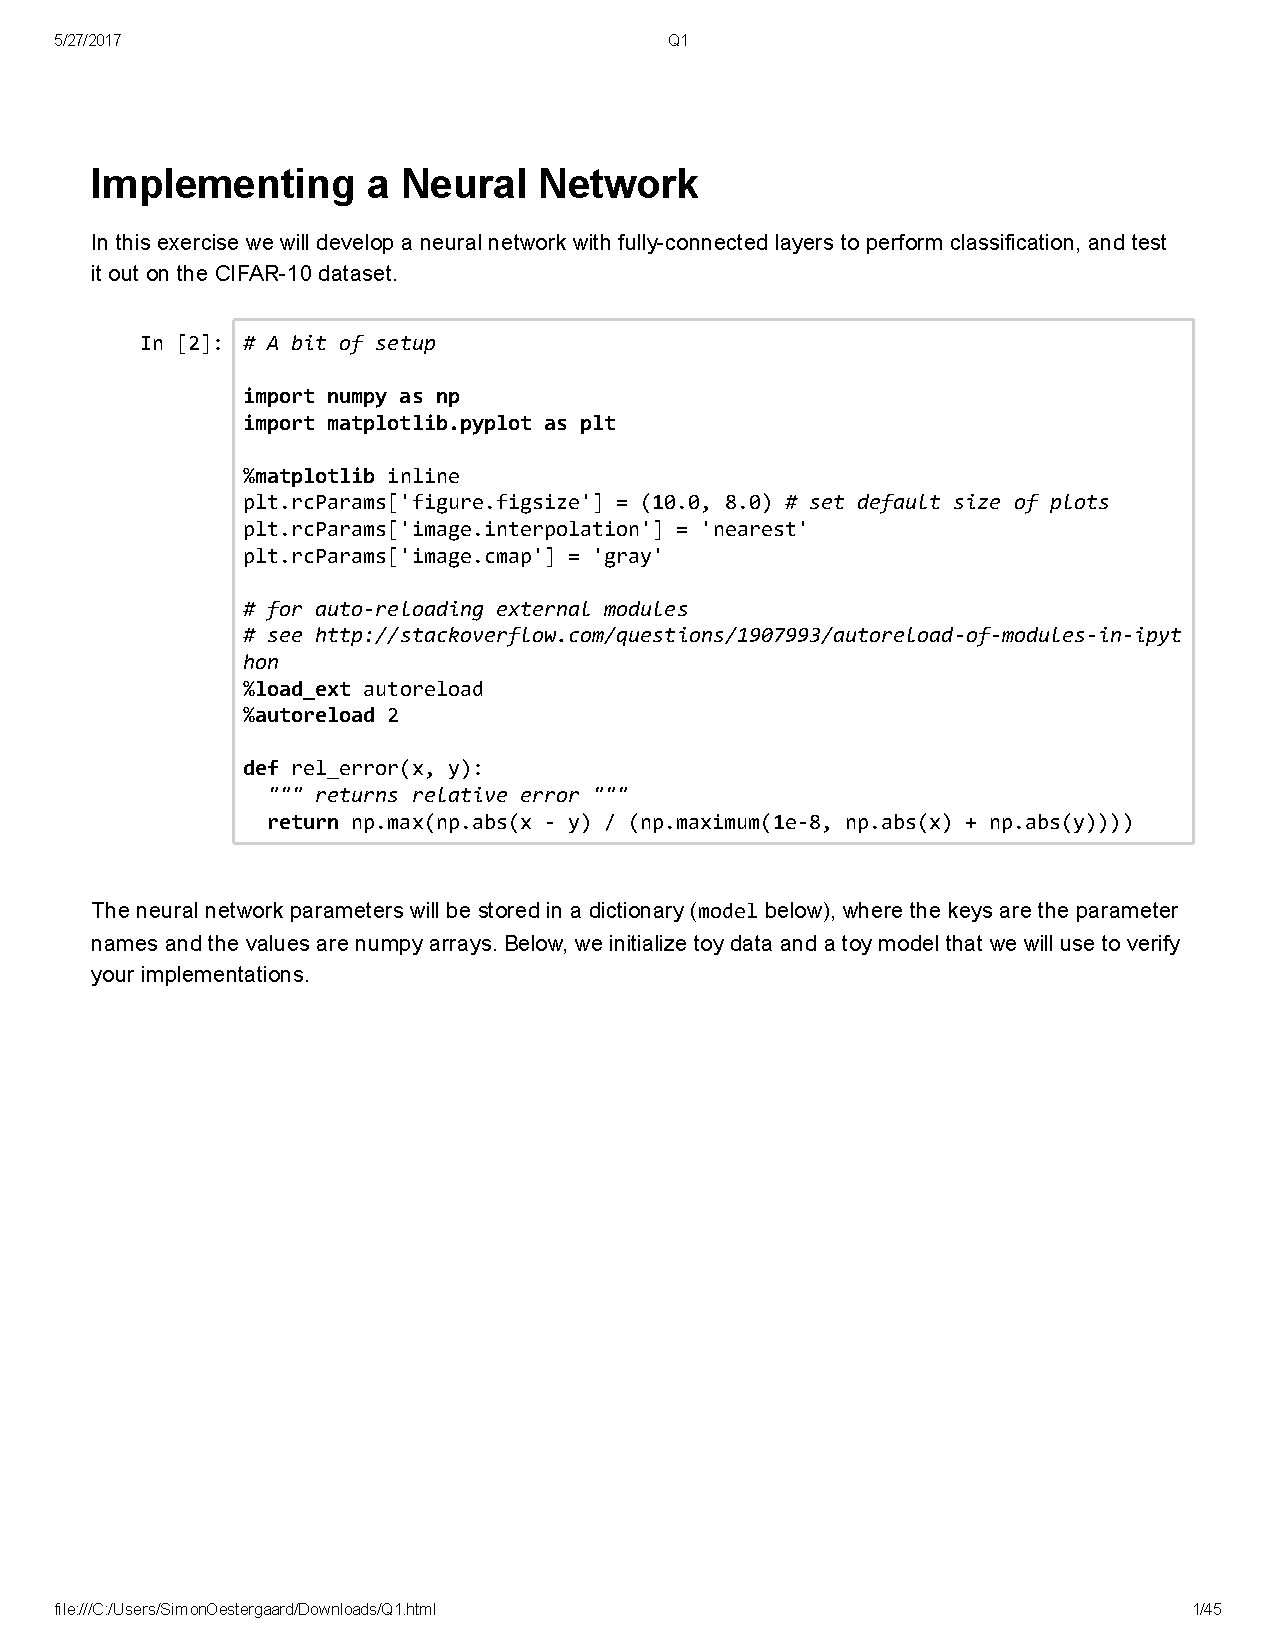
\includepdf[pages={-20}]{chapter/Q1.pdf}
\includepdf[pages={44-}]{chapter/Q1.pdf}
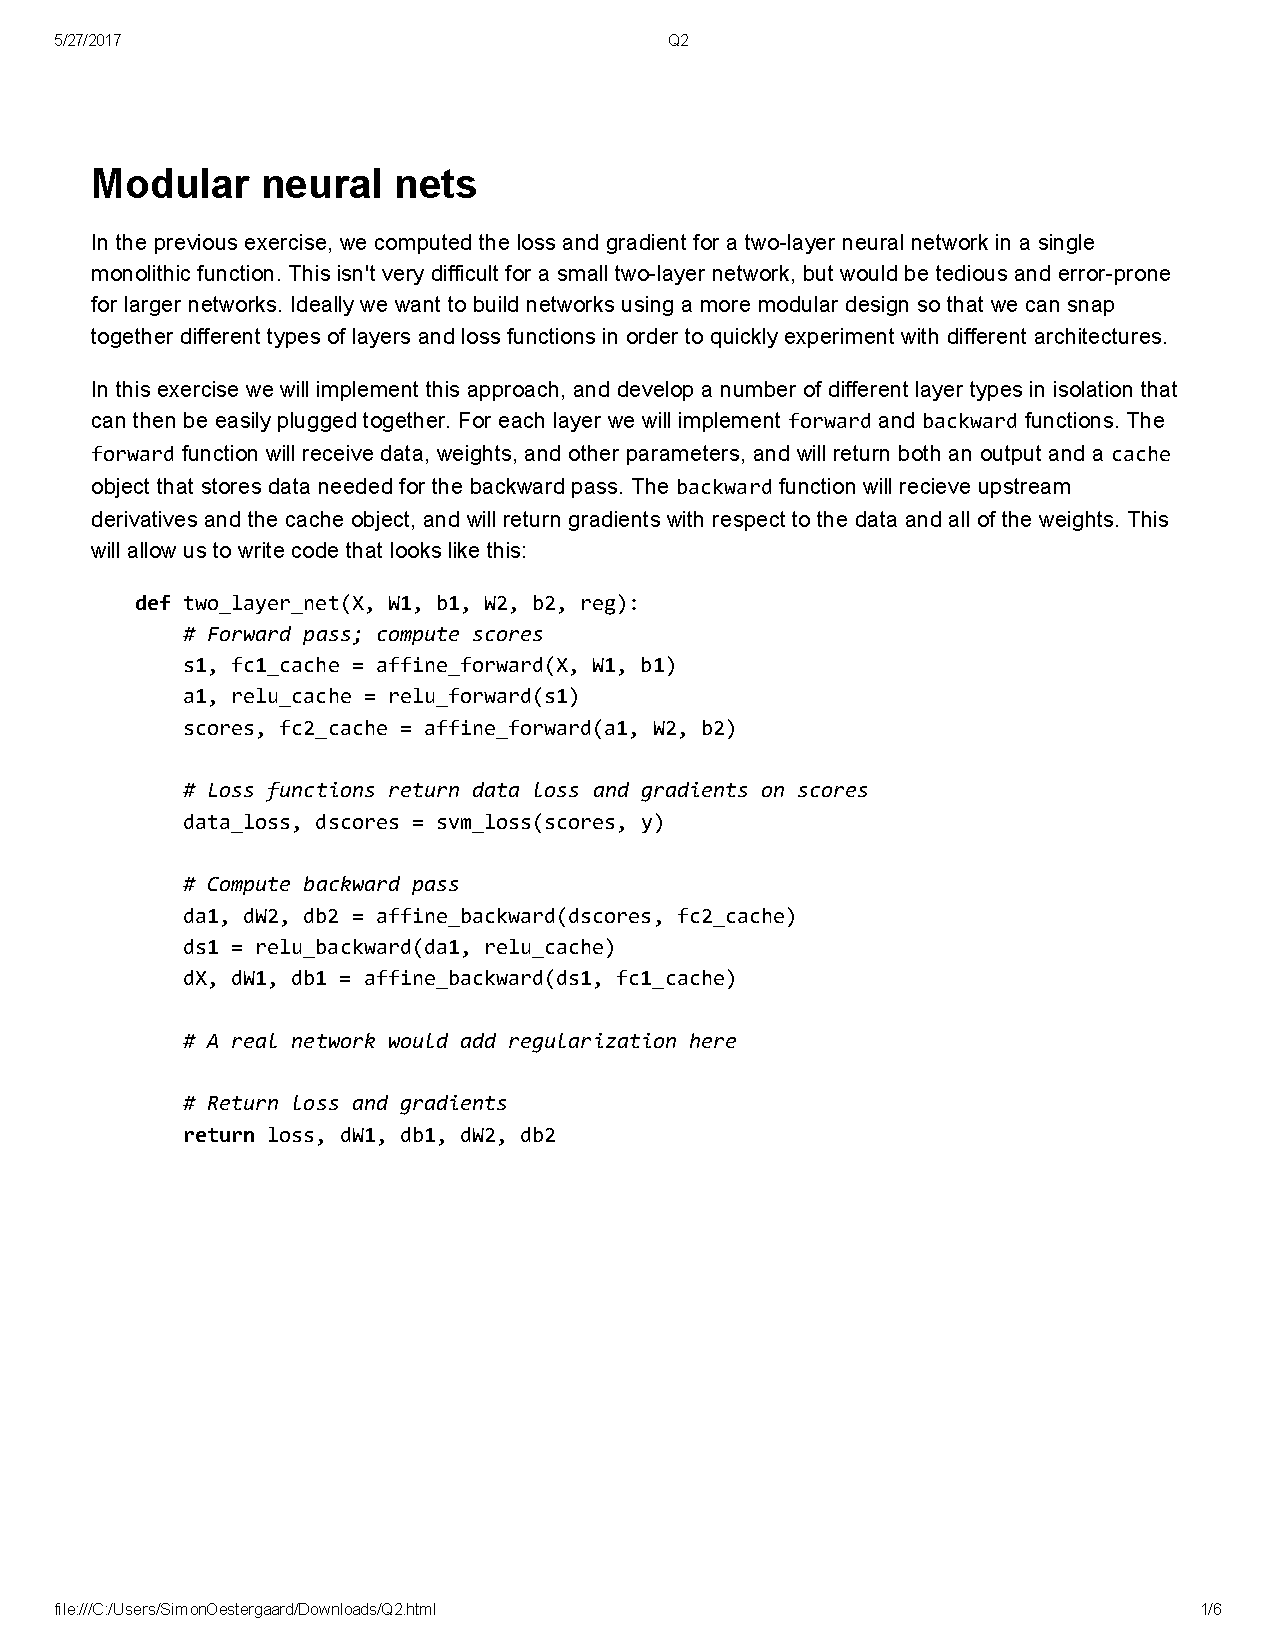
\includepdf[pages={-}]{chapter/Q2.pdf}





\begin{lstlisting}[language=Python, label=lst:neuralnet.py, caption={neural\_net.py}, basicstyle=\tiny]
import numpy as np
import matplotlib.pyplot as plt

def init_two_layer_model(input_size, hidden_size, output_size):
"""
Initialize the weights and biases for a two-layer fully connected neural
network. The net has an input dimension of D, a hidden layer dimension of H,
and performs classification over C classes. Weights are initialized to small
random values and biases are initialized to zero.

Inputs:
- input_size: The dimension D of the input data
- hidden_size: The number of neurons H in the hidden layer
- ouput_size: The number of classes C

Returns:
A dictionary mapping parameter names to arrays of parameter values. It has
the following keys:
- W1: First layer weights; has shape (D, H)
- b1: First layer biases; has shape (H,)
- W2: Second layer weights; has shape (H, C)
- b2: Second layer biases; has shape (C,)
"""
# initialize a model
model = {}
model['W1'] = 0.00001 * np.random.randn(input_size, hidden_size)
model['b1'] = np.zeros(hidden_size)
model['W2'] = 0.00001 * np.random.randn(hidden_size, output_size)
model['b2'] = np.zeros(output_size)
return model

def two_layer_net(X, model, y=None, reg=0.0):
"""
Compute the loss and gradients for a two layer fully connected neural network.
The net has an input dimension of D, a hidden layer dimension of H, and
performs classification over C classes. We use a softmax loss function and L2
regularization the the weight matrices. The two layer net should use a ReLU
nonlinearity after the first affine layer.

The two layer net has the following architecture:

input - fully connected layer - ReLU - fully connected layer - softmax

The outputs of the second fully-connected layer are the scores for each
class.

Inputs:
- X: Input data of shape (N, D). Each X[i] is a training sample.
- model: Dictionary mapping parameter names to arrays of parameter values.
It should contain the following:
- W1: First layer weights; has shape (D, H)
- b1: First layer biases; has shape (H,)
- W2: Second layer weights; has shape (H, C)
- b2: Second layer biases; has shape (C,)
- y: Vector of training labels. y[i] is the label for X[i], and each y[i] is
an integer in the range 0 <= y[i] < C. This parameter is optional; if it
is not passed then we only return scores, and if it is passed then we
instead return the loss and gradients.
- reg: Regularization strength.

Returns:
If y not is passed, return a matrix scores of shape (N, C) where scores[i, c]
is the score for class c on input X[i].

If y is not passed, instead return a tuple of:
- loss: Loss (data loss and regularization loss) for this batch of training
samples.
- grads: Dictionary mapping parameter names to gradients of those parameters
with respect to the loss function. This should have the same keys as model.
"""

# unpack variables from the model dictionary
W1,b1,W2,b2 = model['W1'], model['b1'], model['W2'], model['b2']
N, D = X.shape  
# input - fully connected layer - ReLU - fully connected layer - softmax
#Activation function
reluF = lambda x: np.maximum(0, x)
#Compared to lecture notes we switch X and W1 because to multiple the inputs 
#with the correct weights
h1 = reluF(np.dot(X, W1) + b1)
scores = np.dot(h1, W2) + b2
#############################################################################
#                              END OF YOUR CODE                             #
#############################################################################

# If the targets are not given then jump out, we're done
if y is None:
return scores

#############################################################################
# TODO: Finish the forward pass, and compute the loss. This should include  #
# both the data loss and L2 regularization for W1 and W2. Store the result  #
# in the variable loss, which should be a scalar. Use the Softmax           #
# classifier loss. So that your results match ours, multiply the            #
# regularization loss by 0.5                                                #
#############################################################################
# compute the loss
expScores = np.exp(scores)
rowSum = expScores.sum(axis=1, keepdims=True)
# Normalized scores
propScores = expScores / rowSum
logprob_correctLabel = -np.log(propScores[range(N),y])
softmax_loss = 1/float(N) * np.sum(logprob_correctLabel)
#regulization loss
reg_loss = 0.5 * reg * np.sum(W1*W1) + 0.5 * reg * np.sum(W2 * W2)
#Final loss 
loss = softmax_loss + reg_loss
#############################################################################
#                              END OF YOUR CODE                             #
#############################################################################

# compute the gradients
grads = {}

#############################################################################
# TODO: Compute the backward pass, computing the derivatives of the weights #
# and biases. Store the results in the grads dictionary. For example,       #
# grads['W1'] should store the gradient on W1, and be a matrix of same size #
#############################################################################
# Firstly we calculate the gradient on the scores.
# The gradient from the loss function is simply -1.
# This is subtracted from the correct scores for each
# dscores are the probabilities for all classes as a row for each sample
dscores = propScores
#For each row(sample) in dscores 1 is subtracted from the correct element 
#specified by y
dscores[range(N),y] -= 1
# We then divide all elements with N(number of samples)
dscores /= N

# The gradient for W2 is simply the output from the RELU activation function (h1)
# multiplyed with the dscores that contains the gradient on the scores.
# d/dw(w*x) = x which is our h1 then we get the input times dscores
grads['W2'] = np.dot(h1.T, dscores)
#bias is just the sum of the dscores
grads['b2'] = np.sum(dscores, axis=0)

# next backprop into hidden layer. This is the scores multiplied with the weights
# for second layer
dhidden = np.dot(dscores, W2.T)
# backprop the ReLU non-linearity. 
#For elements < or equals 0  we set them equals to 0
# remember how Relu is just max, so it routes the gradients
dhidden[h1 <= 0] = 0
# same thing as second layer - d/dw(w*x) = x, so x times our gradient for dhidden
grads['W1'] = np.dot(X.T, dhidden)
grads['b1'] = np.sum(dhidden, axis=0)

# adding gradient for regulization
# d/dw(1/2*reg*W1*w1) = reg * W1
grads['W1'] += reg * W1 
grads['W2'] += reg * W2
#############################################################################
#                              END OF YOUR CODE                             #
#############################################################################

return loss, grads
\end{lstlisting}










\begin{lstlisting}[language=Python, label=lst:classifiertrainer.py, caption={classifier\_trainer.py}, basicstyle=\tiny]
import numpy as np


class ClassifierTrainer(object):
""" The trainer class performs SGD with momentum on a cost function """
def __init__(self):
self.step_cache = {} # for storing velocities in momentum update

def train(self, X, y, X_val, y_val, 
model, loss_function, 
reg=0.0,
learning_rate=1e-2, momentum=0, learning_rate_decay=0.95,
update='momentum', sample_batches=True,
num_epochs=30, batch_size=100, acc_frequency=None,
verbose=False):
"""
Optimize the parameters of a model to minimize a loss function. We use
training data X and y to compute the loss and gradients, and periodically
check the accuracy on the validation set.

Inputs:
- X: Array of training data; each X[i] is a training sample.
- y: Vector of training labels; y[i] gives the label for X[i].
- X_val: Array of validation data
- y_val: Vector of validation labels
- model: Dictionary that maps parameter names to parameter values. Each
parameter value is a numpy array.
- loss_function: A function that can be called in the following ways:
scores = loss_function(X, model, reg=reg)
loss, grads = loss_function(X, model, y, reg=reg)
- reg: Regularization strength. This will be passed to the loss function.
- learning_rate: Initial learning rate to use.
- momentum: Parameter to use for momentum updates.
- learning_rate_decay: The learning rate is multiplied by this after each
epoch.
- update: The update rule to use. One of 'sgd', 'momentum', or 'rmsprop'.
- sample_batches: If True, use a minibatch of data for each parameter update
(stochastic gradient descent); if False, use the entire training set for
each parameter update (gradient descent).
- num_epochs: The number of epochs to take over the training data.
- batch_size: The number of training samples to use at each iteration.
- acc_frequency: If set to an integer, we compute the training and
validation set error after every acc_frequency iterations.
- verbose: If True, print status after each epoch.

Returns a tuple of:
- best_model: The model that got the highest validation accuracy during
training.
- loss_history: List containing the value of the loss function at each
iteration.
- train_acc_history: List storing the training set accuracy at each epoch.
- val_acc_history: List storing the validation set accuracy at each epoch.
"""

N = X.shape[0]

if sample_batches:
iterations_per_epoch = N / batch_size # using SGD
else:
iterations_per_epoch = 1 # using GD
num_iters = num_epochs * iterations_per_epoch
epoch = 0
best_val_acc = 0.0
best_model = {}
loss_history = []
train_acc_history = []
val_acc_history = []
for it in xrange(num_iters):
if it % 10 == 0:  print 'starting iteration ', it

# get batch of data
if sample_batches:
batch_mask = np.random.choice(N, batch_size)
X_batch = X[batch_mask]
y_batch = y[batch_mask]
else:
# no SGD used, full gradient descent
X_batch = X
y_batch = y

# evaluate cost and gradient
cost, grads = loss_function(X_batch, model, y_batch, reg)
loss_history.append(cost)

# perform a parameter update
for p in model:
# compute the parameter step
if update == 'sgd':
dx = -learning_rate * grads[p]
elif update == 'momentum':
if not p in self.step_cache: 
self.step_cache[p] = np.zeros(grads[p].shape)
dx = np.zeros_like(grads[p]) # you can remove this after
#####################################################################
# TODO: implement the momentum update formula and store the step    #
# update into variable dx. You should use the variable              #
# step_cache[p] and the momentum strength is stored in momentum.    #
# Don't forget to also update the step_cache[p].                    #
#####################################################################
# Momentum update
# Momentum strength is a coefficient explains to friction,
# moment strength damps velocity and reduces the kinetic energy
#it ensures that the particle stops at the bottom
# step_cache is our velocity at time t-1
# From that we subtract the learning rate multiplied the gradients, 
# because we go in the opposite direction of the gradient
dx = momentum * self.step_cache[p] - learning_rate * grads[p] # integrate velocity
self.step_cache[p] = dx 

#####################################################################
#                      END OF YOUR CODE                             #
#####################################################################
elif update == 'rmsprop':
decay_rate = 0.99 # you could also make this an option
if not p in self.step_cache: 
self.step_cache[p] = np.zeros(grads[p].shape)
#####################################################################
# TODO: implement the RMSProp update and store the parameter update #
# dx. Don't forget to also update step_cache[p]. Use smoothing 1e-8 #
#####################################################################
#eps = 1e-8
eps = 1e5
self.step_cache[p] = decay_rate * self.step_cache[p] + (1 - decay_rate) * grads[p]**2
dx = - learning_rate * grads[p] / (np.sqrt(self.step_cache[p]) + eps)


#####################################################################
#                      END OF YOUR CODE                             #
#####################################################################
else:
raise ValueError('Unrecognized update type "%s"' % update)

# update the parameters
model[p] += dx

# every epoch perform an evaluation on the validation set
first_it = (it == 0)
epoch_end = (it + 1) % iterations_per_epoch == 0
acc_check = (acc_frequency is not None and it % acc_frequency == 0)
if first_it or epoch_end or acc_check:
if it > 0 and epoch_end:
# decay the learning rate
learning_rate *= learning_rate_decay
epoch += 1

# evaluate train accuracy
if N > 1000:
train_mask = np.random.choice(N, 1000)
X_train_subset = X[train_mask]
y_train_subset = y[train_mask]
else:
X_train_subset = X
y_train_subset = y
scores_train = loss_function(X_train_subset, model)
y_pred_train = np.argmax(scores_train, axis=1)
train_acc = np.mean(y_pred_train == y_train_subset)
train_acc_history.append(train_acc)

# evaluate val accuracy
scores_val = loss_function(X_val, model)
y_pred_val = np.argmax(scores_val, axis=1)
val_acc = np.mean(y_pred_val ==  y_val)
val_acc_history.append(val_acc)

# keep track of the best model based on validation accuracy
if val_acc > best_val_acc:
# make a copy of the model
best_val_acc = val_acc
best_model = {}
for p in model:
best_model[p] = model[p].copy()

# print progress if needed
if verbose:
print ('Finished epoch %d / %d: cost %f, train: %f, val %f, lr %e'
% (epoch, num_epochs, cost, train_acc, val_acc, learning_rate))

if verbose:
print 'finished optimization. best validation accuracy: %f' % (best_val_acc, )
# return the best model and the training history statistics
return best_model, loss_history, train_acc_history, val_acc_history
\end{lstlisting}









\begin{lstlisting}[language=Python, label=lst:layers.py, caption={layers.py}, basicstyle=\tiny]
import numpy as np

def affine_forward(x, w, b):
"""
Computes the forward pass for an affine (fully-connected) layer.

The input x has shape (N, d_1, ..., d_k) where x[i] is the ith input.
We multiply this against a weight matrix of shape (D, M) where
D = \prod_i d_i

Inputs:
x - Input data, of shape (N, d_1, ..., d_k)
w - Weights, of shape (D, M)
b - Biases, of shape (M,)

Returns a tuple of:
- out: output, of shape (N, M)
- cache: (x, w, b)
"""
out = None
#############################################################################
# TODO: Implement the affine forward pass. Store the result in out. You     #
# will need to reshape the input into rows.                                 #
#############################################################################
# First we reshape X to mulitply it with the incoming weights
# We get column and row size and then reshape
row_size = x.shape[0]
col_size = np.prod(x.shape[1:])
x_reshape = x.reshape(row_size, col_size)
# To execute the forward pass we simply need to multiply the inputs with the weights
out = np.dot(x_reshape, w) + b
#############################################################################
#                             END OF YOUR CODE                              #
#############################################################################
cache = (x, w, b)
return out, cache


def affine_backward(dout, cache):
"""
Computes the backward pass for an affine layer.

Inputs:
- dout: Upstream derivative, of shape (N, M)
- cache: Tuple of:
- x: Input data, of shape (N, d_1, ... d_k)
- w: Weights, of shape (D, M)

Returns a tuple of:
- dx: Gradient with respect to x, of shape (N, d1, ..., d_k)
- dw: Gradient with respect to w, of shape (D, M)
- db: Gradient with respect to b, of shape (M,)
"""
x, w, b = cache
dx, dw, db = None, None, None
#############################################################################
# TODO: Implement the affine backward pass.                                 #
#############################################################################
# First we reshape X to mulitply it with the incoming weights
# We get column and row size and then reshape
row_size = x.shape[0]
col_size = np.prod(x.shape[1:])
x_reshape = x.reshape(row_size, col_size)

# After reshaping we calculate the backward pass

# Gradient with respect to x
# Gradient of x*w with respect to x is simply w, 
# We multiply that with the upstream gradient
dx2 = np.dot(dout, w.T) 
dx = np.reshape(dx2, x.shape)

# Gradient with respect to weights
# Gradient of x*w with respect to w is simply x,
# We multiply that with the upstream gradient
dw = np.dot(x_reshape.T, dout)

# Gradient with respect to bias
# Biases are added so the gradient is simply 1,
# We multiply that with the upstream gradient.
db = np.dot(dout.T, np.ones(row_size))

#############################################################################
#                             END OF YOUR CODE                              #
#############################################################################
return dx, dw, db


def relu_forward(x):
"""
Computes the forward pass for a layer of rectified linear units (ReLUs).

Input:
- x: Inputs, of any shape

Returns a tuple of:
- out: Output, of the same shape as x
- cache: x
"""
out = None
#############################################################################
# TODO: Implement the ReLU forward pass.                                    #
#############################################################################
reluF = lambda x: np.maximum(0, x)
out = reluF(x)
#############################################################################
#                             END OF YOUR CODE                              #
#############################################################################
cache = x
return out, cache


def relu_backward(dout, cache):
"""
Computes the backward pass for a layer of rectified linear units (ReLUs).

Input:
- dout: Upstream derivatives, of any shape
- cache: Input x, of same shape as dout

Returns:
- dx: Gradient with respect to x
"""
dx, x = None, cache
#############################################################################
# TODO: Implement the ReLU backward pass.                                   #
#############################################################################
#reluf function
reluF = lambda x: np.maximum(0, x)

out = reluF(x)
# Reluf is a max gate and so we can think of it as a router of gradients
# the max value is the one that the gradient is routated to
# we simpy set the out value to 1 if the out value is bigger than 0
out[out > 0] = 1

# Multiply out  with upstream gradient, to "route" the gradient
dx = out * dout
#############################################################################
#                             END OF YOUR CODE                              #
#############################################################################
return dx

def dropout_forward(x, dropout_param):
"""
Performs the forward pass for (inverted) dropout.

Inputs:
- x: Input data, of any shape
- dropout_param: A dictionary with the following keys:
- p: Dropout parameter. We keep each neuron output with probability p.
- mode: 'test' or 'train'. If the mode is train, then perform dropout;
if the mode is test, then just return the input.
- seed: Seed for the random number generator. Passing seed makes this
function deterministic, which is needed for gradient checking but not in
real networks.

Outputs:
- out: Array of the same shape as x.
- cache: A tuple (dropout_param, mask). In training mode, mask is the dropout
mask that was used to multiply the input; in test mode, mask is None.
"""
p, mode = dropout_param['p'], dropout_param['mode']
if 'seed' in dropout_param:
np.random.seed(dropout_param['seed'])

mask = None
out = None

if mode == 'train':
###########################################################################
# TODO: Implement the training phase forward pass for inverted dropout.   #
# Store the dropout mask in the mask variable.                            #
###########################################################################
pass
###########################################################################
#                            END OF YOUR CODE                             #
###########################################################################
elif mode == 'test':
###########################################################################
# TODO: Implement the test phase forward pass for inverted dropout.       #
###########################################################################
pass
###########################################################################
#                            END OF YOUR CODE                             #
###########################################################################

cache = (dropout_param, mask)
out = out.astype(x.dtype, copy=False)

return out, cache


def dropout_backward(dout, cache):
"""
Perform the backward pass for (inverted) dropout.

Inputs:
- dout: Upstream derivatives, of any shape
- cache: (dropout_param, mask) from dropout_forward.
"""
dropout_param, mask = cache
mode = dropout_param['mode']
if mode == 'train':
###########################################################################
# TODO: Implement the training phase forward pass for inverted dropout.   #
# Store the dropout mask in the mask variable.                            #
###########################################################################
pass
###########################################################################
#                            END OF YOUR CODE                             #
###########################################################################
elif mode == 'test':
dx = dout
return dx


def conv_forward_naive(x, w, b, conv_param):
"""
A naive implementation of the forward pass for a convolutional layer.

The input consists of N data points, each with C channels, height H and width
W. We convolve each input with F different filters, where each filter spans
all C channels and has height HH and width HH.

Input:
- x: Input data of shape (N, C, H, W)
- w: Filter weights of shape (F, C, HH, WW)
- b: Biases, of shape (F,)
- conv_param: A dictionary with the following keys:
- 'stride': The number of pixels between adjacent receptive fields in the
horizontal and vertical directions.
- 'pad': The number of pixels that will be used to zero-pad the input.

Returns a tuple of:
- out: Output data, of shape (N, F, H', W') where H' and W' are given by
H' = 1 + (H + 2 * pad - HH) / stride
W' = 1 + (W + 2 * pad - WW) / stride
- cache: (x, w, b, conv_param)
"""
out = None
#############################################################################
# TODO: Implement the convolutional forward pass.                           #
# Hint: you can use the function np.pad for padding.                        #
#############################################################################
pass
#############################################################################
#                             END OF YOUR CODE                              #
#############################################################################
cache = (x, w, b, conv_param)
return out, cache


def conv_backward_naive(dout, cache):
"""
A naive implementation of the backward pass for a convolutional layer.

Inputs:
- dout: Upstream derivatives.
- cache: A tuple of (x, w, b, conv_param) as in conv_forward_naive

Returns a tuple of:
- dx: Gradient with respect to x
- dw: Gradient with respect to w
- db: Gradient with respect to b
"""
dx, dw, db = None, None, None
#############################################################################
# TODO: Implement the convolutional backward pass.                          #
#############################################################################
pass
#############################################################################
#                             END OF YOUR CODE                              #
#############################################################################
return dx, dw, db


def max_pool_forward_naive(x, pool_param):
"""
A naive implementation of the forward pass for a max pooling layer.

Inputs:
- x: Input data, of shape (N, C, H, W)
- pool_param: dictionary with the following keys:
- 'pool_height': The height of each pooling region
- 'pool_width': The width of each pooling region
- 'stride': The distance between adjacent pooling regions

Returns a tuple of:
- out: Output data
- cache: (x, pool_param)
"""
out = None
#############################################################################
# TODO: Implement the max pooling forward pass                              #
#############################################################################
pass
#############################################################################
#                             END OF YOUR CODE                              #
#############################################################################
cache = (x, pool_param)
return out, cache


def max_pool_backward_naive(dout, cache):
"""
A naive implementation of the backward pass for a max pooling layer.

Inputs:
- dout: Upstream derivatives
- cache: A tuple of (x, pool_param) as in the forward pass.

Returns:
- dx: Gradient with respect to x
"""
dx = None
#############################################################################
# TODO: Implement the max pooling backward pass                             #
#############################################################################
pass
#############################################################################
#                             END OF YOUR CODE                              #
#############################################################################
return dx


def svm_loss(x, y):
"""
Computes the loss and gradient using for multiclass SVM classification.

Inputs:
- x: Input data, of shape (N, C) where x[i, j] is the score for the jth class
for the ith input.
- y: Vector of labels, of shape (N,) where y[i] is the label for x[i] and
0 <= y[i] < C

Returns a tuple of:
- loss: Scalar giving the loss
- dx: Gradient of the loss with respect to x
"""
N = x.shape[0]
correct_class_scores = x[np.arange(N), y]
margins = np.maximum(0, x - correct_class_scores[:, np.newaxis] + 1.0)
margins[np.arange(N), y] = 0
loss = np.sum(margins) / N
num_pos = np.sum(margins > 0, axis=1)
dx = np.zeros_like(x)
dx[margins > 0] = 1
dx[np.arange(N), y] -= num_pos
dx /= N
return loss, dx


def softmax_loss(x, y):
"""
Computes the loss and gradient for softmax classification.

Inputs:
- x: Input data, of shape (N, C) where x[i, j] is the score for the jth class
for the ith input.
- y: Vector of labels, of shape (N,) where y[i] is the label for x[i] and
0 <= y[i] < C

Returns a tuple of:
- loss: Scalar giving the loss
- dx: Gradient of the loss with respect to x
"""
probs = np.exp(x - np.max(x, axis=1, keepdims=True))
probs /= np.sum(probs, axis=1, keepdims=True)
N = x.shape[0]
loss = -np.sum(np.log(probs[np.arange(N), y])) / N
dx = probs.copy()
dx[np.arange(N), y] -= 1
dx /= N
return loss, dx
\end{lstlisting}
    \chapter{Exercise 2}

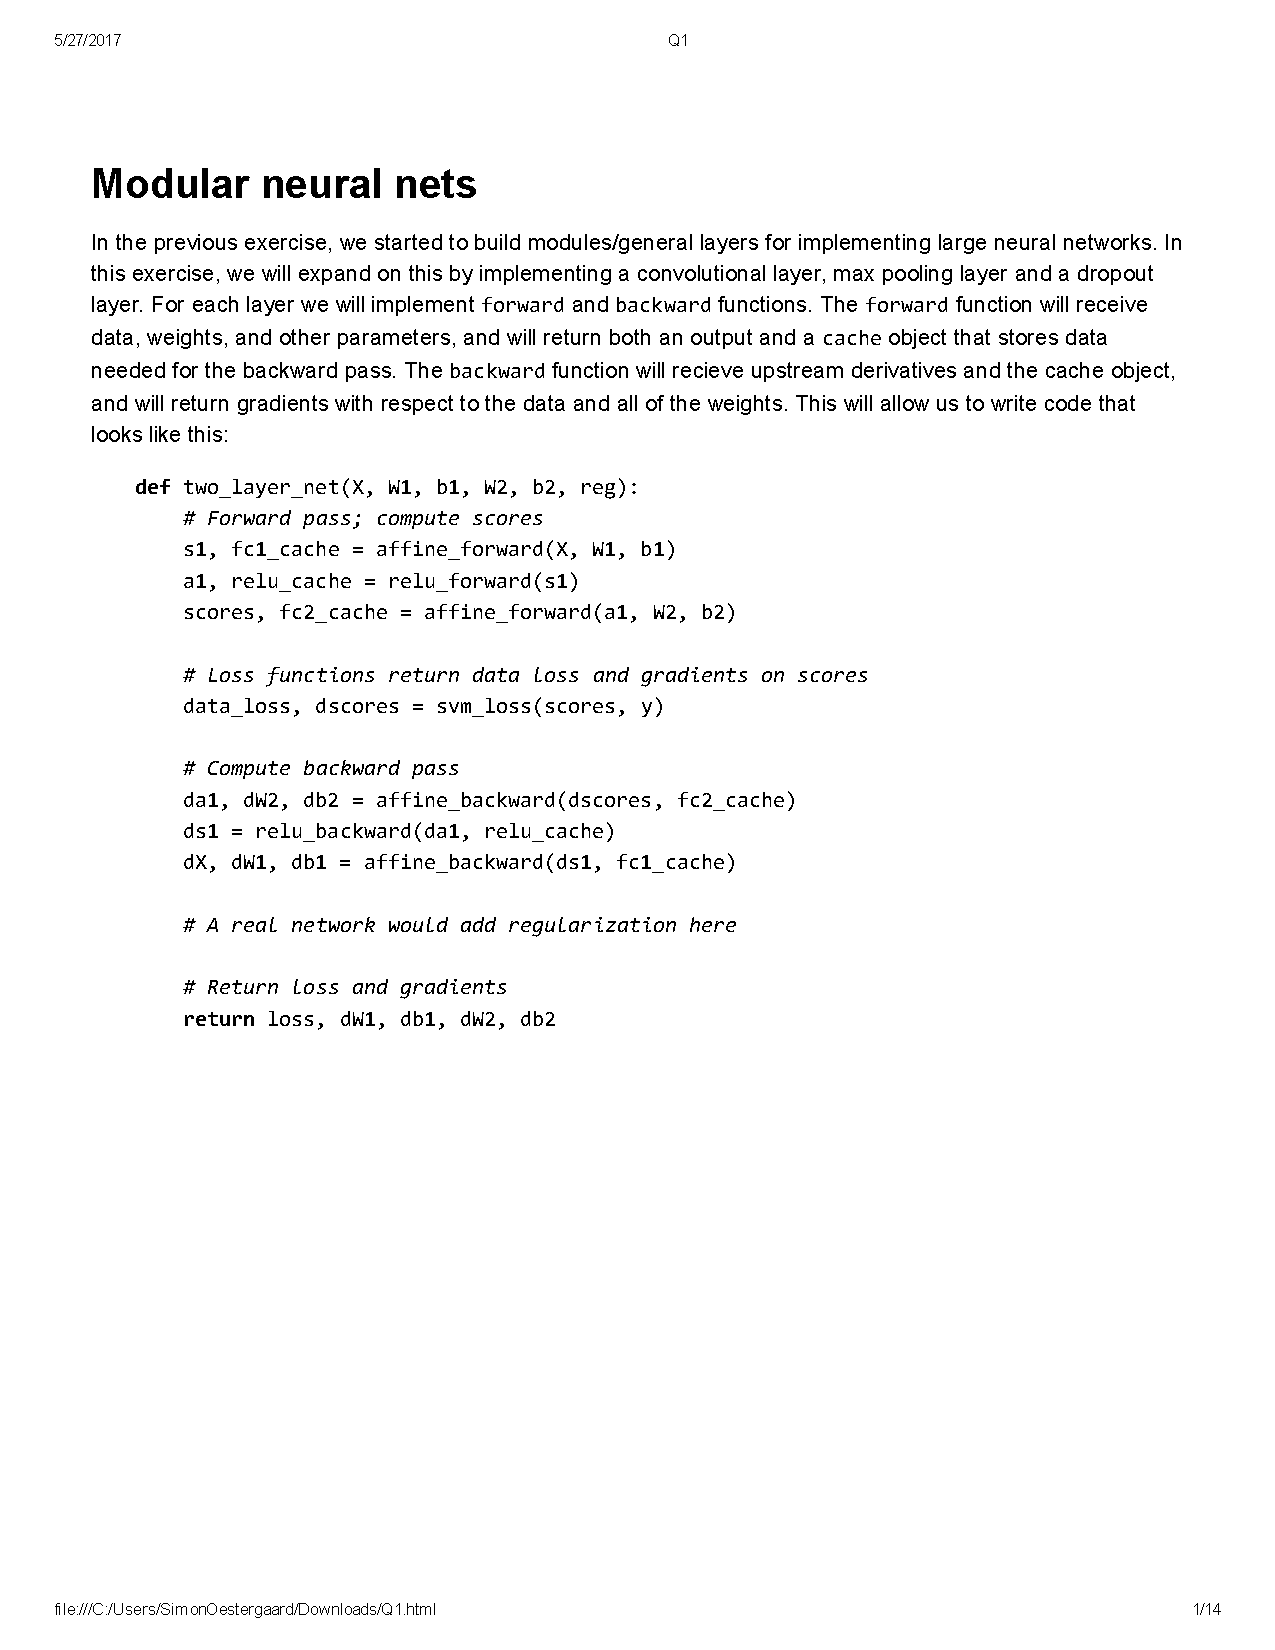
\includepdf[pages={-}]{chapter/2_Q1.pdf}


%	\addtocontents{toc}{\protect\setcounter{tocdepth}1}
%	\addtocontents{toc}{\setcounter{tocdepth}{1}}
    
    % Appendix
    \appendix


% Adding appendix to toc and setting space between "Bilag A" and "chapter name"
\addtocontents{toc}{\setlength\cftchapternumwidth{1cm}}

% Redifining chapterstyle for appendix(document past this point)
\chapterstyle{default}
% Changing vertical position of chapter headline
\renewcommand*{\chapterheadstart}{\vspace*{-20pt}}

% Section numbers in margin
%\defaultsecnum
\hangsecnum

% Color setup for sections
% Title color
\renewcommand\thesection{\thechapter.\arabic{section}}

% Set the depth of sections included in table of contents
\settocdepth{chapter} % Changes chapter and section style and toc adding
    

\end{document}
